\section{Context and Motivation}

%. Over the last decade, a popular modification to the DBSCAN algorithm, HDBSCAN \cite{rahman2016hdbscandensitybasedclustering}, has also shown prowess in clustering-based anomaly detection \cite{ariyaluran2022clustering}

\subsection{Context} 

\acrshort{das} is a technology that enables real-time acoustic sensing along fiber-optic cables by analyzing Rayleigh backscattering. Based on \acrfull{potdr} \cite{s16050681}, the system sends light pulses through the fiber and detects the returned light backscattered from imperfections along its length, as shown in Figure \ref{fig:das-fig}. By analyzing changes in this backscattered light, \acrshort{das} can detect and localize acoustic disturbances along the entire fiber \cite{shang2016optical}. Due to its high sensitivity, \acrshort{das} has gained recognition over the last decade for detecting subtle environmental changes and anomalies. It has applications in various fields, including landslide and earthquake detection and railroad and maritime monitoring. Effective and efficient processing and interpretation of \acrshort{das} data is crucial for extracting meaningful insights from these complex measurements in real-time environments.

\begin{figure}[!h]
    \centering
    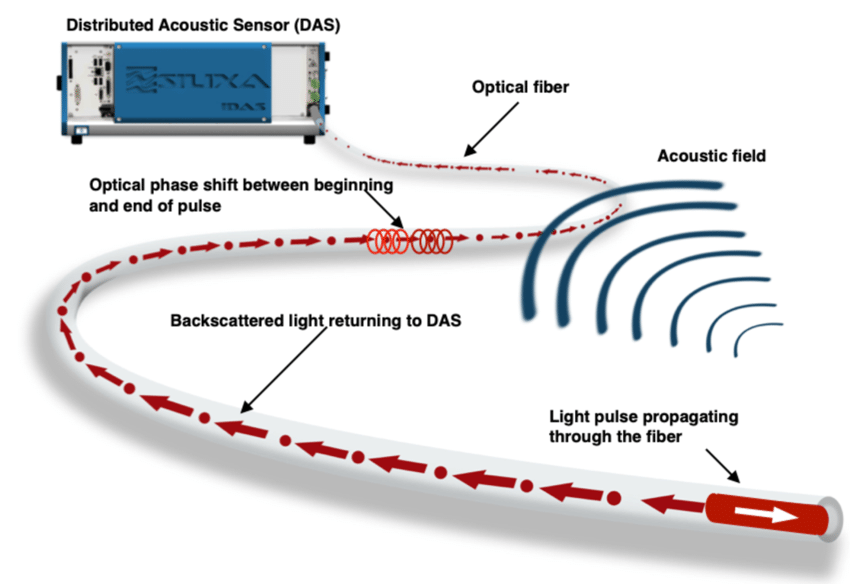
\includegraphics[width=0.7\linewidth]{figures/das.png}
    \caption{Demonstration of how \acrshort{das} works. Light is propagated through the optical fiber, where the backscattered light is returned to the sensor. \footnotemark}
    \label{fig:das-fig}
\end{figure}

\footnotetext{\label{fn:das-image-source}Image source: \url{https://www.researchgate.net/publication/344127365/figure/fig1/AS:1073735670960128@1633009941244/Operation-principle-of-Distributed-Acoustic-Sensing-DAS.png}}

Anomaly detection algorithms for \acrshort{das} data present a varied challenge due to the \textit{spatio-temporal} aspect of the data. \acrshort{das} data can be viewed as multi-channel time series or images, where the spatial features of either the time or frequency domain are studied. The objective of anomaly detection on \acrshort{das} data, in either case, is to find groups or points of irregular signals that differ significantly from the rest of the recorded data. In addition, noise in \acrshort{das} signals presents an additional challenge, where an effective algorithm must differentiate noisy signals from true anomalous signals or have the data denoised before or during training and analysis.

Unsupervised \acrfull{dnn} offer great benefits for anomaly detection in \acrshort{das} due to their more unbiased approach to learning, making them adept at detecting several types of anomalies \cite{wei2022lstmautoencoder, srivastava2016unsupervised}, compared to supervised alternatives. Additionally, not having to label datasets imposes yet another benefit in terms of \acrshort{das} analysis. Among unsupervised \acrshort{dnn}s, autoencoders have been proven particularly efficient for detecting anomalies in \acrshort{das} data CITE. Autoencoders are neural networks designed to learn efficient data codings unsupervised, making them well-suited for dimensionality reduction and anomaly detection in complex, high-dimensional datasets like those produced by \acrshort{das} systems. Recent advancements in unsupervised anomaly detection in \acrshort{das} data try to analyze the entire \textit{spatio-temporal} aspect by combing layers suited for both dimensions CITE.

\subsection{Motivating challenges}

\acrshort{cgf} currently expends considerable time and resources on processing and analyzing \acrshort{das} data. Existing tools are predominantly sequential, and not necessarily optimized for efficiency or memory consumption. This approach limits the volume of data that can be processed simultaneously, leading to inefficiencies in handling the large-scale datasets typical in \acrshort{das} experiments. 
While languages such as Python and Matlab are commonly used for both processing and analysis, these languages may not be optimal for data-intensive applications without integrating lower-level languages like C. Julia, a relatively new language designed for both data science and \acrfull{hpc}, offers a promising alternative. Its potential for developing scalable \acrshort{das} processing applications remains largely unexplored despite its suitability for handling large-scale scientific computations efficiently. 

Furthermore, although numerous autoencoder models exist for \acrshort{das} data analysis, many fail to prioritize memory efficiency or computational complexity. This oversight is particularly problematic for real-time environments, where rapid processing of large data volumes is crucial. There is a clear need for more models that balance analytical power with computational efficiency. 

The \acrshort{das} research field suffers from a lack of free and open-source datasets and open access to \acrshort{ai} models for comparisons and becnhmarks. This is partly due to \acrshort{das} often recording confidential data. This scarcity hinders research progress and reproducibility. Developing open-source programs for training different kinds of \acrshort{dnn}s on \acrshort{das} data could significantly advance the field by providing accessible tools and benchmarks for the field. Despite the promising potential of unsupervised \acrshort{dl} models for anomaly detection in \acrshort{das} data, their application at \acrshort{cgf} remains limited. This represents a missed opportunity for enhancing the efficiency and accuracy of \acrshort{das} data analysis, particularly in identifying complex patterns and anomalies that traditional methods might overlook.

Addressing these challenges could substantially improve the processing and analysis of \acrshort{das} data, leading to more efficient utilization of resources, enhanced real-time capabilities, and broader accessibility of advanced analytical tools in the field. 

%The overarching question this thesis tries to answer is as follows: ''How can we make the entire data processing pipeline, from loading \acrshort{das} data to detecting anomalies, as fast and efficient as possible?''.

